\documentclass[chaptersright]{informeutn}
\usepackage{circuitikz}
\usepackage{amssymb}
\tikzset{every picture/.style={line width=0.75pt}} %set default line width to 0.75pt        

% Datos del informe
\materia{Electrónica Aplicada I}
\titulo{Trabajo Práctico 3}
\comision{3R2}
\autores{
          Gaston Grasso - 401892\\
          Franco Palombo - 401910\\
          Angelo Prieto - 401012}
\fecha{20/08/2025}

\begin{document}
  \maketitle
  \tableofcontents
  \setcounter{page}{1}
  \thispagestyle{plain}

\chapter{Introducción}

\chapter{Diseño para Máxima Excursión Simétrica}
En la Figura \ref{fig:amplificador} se muestra el circuito utilizado en el presente trabajo práctico. El mismo consiste
en un amplificador basado en un transistor BJT en configuración emisor común con 
polarización mediante divisor resistivo. Esta topología se caracteriza por permitir un punto de operación
estable frente a variaciones del $\beta$. 
El circuito incluye las resistencias $R_1$, $R_2$, $R_E$, $R_C$ y $R_L$, junto a capacitores de desacople y una fuente de 
alimentación $V_{CC}$. Algunos de estos valores fueron fijados por las consignas del trabajo.

\begin{figure}[!ht]
    \centering
    \begin{tikzpicture}
      \node[npn](N1) at (9.25, 5.75){} node[anchor=west] at (N1.text){$Q1$};
      \draw (7, 5) to[american resistor, l={$R_1$}] (7, 2.75);
      \draw (7, 5.75) to[capacitor, l={$C_1$}] (3, 5.75);
      \draw (7, 5.75) -- (8.41, 5.75);
      \draw (9.25, 5) to[american resistor, l={$R_E$}] (9.25, 2.75);
      \draw (3, 5.75) to[sinusoidal voltage source, l={$v_i$}] (3, 2.5);
      \draw (7, 8.75) to[american resistor, l={$R_2$}, name=R1] (7, 6.5);
      \draw (9.25, 8.77) to[american resistor, l={$R_C$}] (9.25, 6.52);
      \draw (7, 5) -| (7, 6.5);
      \draw (11, 5) to[capacitor, l={$C_E$}] (11, 2.75);
      \draw (9.25, 5) -- (11, 5);
      \draw (7, 8.75) -| (7, 9) -| (9.25, 8.77);
      \draw (11, 2.75) |- (7, 2.5) -| (7, 2.75);
      \draw (9.25, 2.75) -| (9.25, 2.5);
      \draw (3, 2.5) -- (7, 2.5);
      \draw (10.25, 6.5) to[capacitor, l={$C_2$}] (13, 6.5);
      \draw (13.75, 5.5) to[american resistor, l={$R_L$}] (13.75, 3.25);
      \draw (13.75, 6.5) -| (13.75, 5.5);
      \draw (11, 2.5) -| (13.75, 3.25);
      \node[vcc](N2) at (9.25, 9.75){} node[anchor=south] at (N2.text){$V_{CC}$};
      \draw (9.25, 9) -| (9.25, 9.75);
      \node[ground] at (9.25, 2){};
      \draw (9.25, 2.5) -| (9.25, 2);
      \draw (10.25, 6.5) -- (9.25, 6.5);
      \draw (13, 6.5) -- (13.75, 6.5);
    \end{tikzpicture}
    \caption{amplificador emisor común.}
    \label{fig:amplificador}
\end{figure}

El objetivo de esta sección es establecer las condiciones de polarización en corriente continua de 
manera que el transistor opere en la región activa, garantizando linealidad en la 
amplificación de señales pequeñas. En particular, se busca ubicar el punto de operación $Q$ 
en la recta de carga de tal forma que la señal de salida pueda desplazarse con la mayor 
amplitud posible antes de alcanzar las regiones de saturación o corte.

Este criterio se conoce como polarización para máxima excursión simétrica (MES). Consiste 
en ajustar el punto de operación en el centro de las características de salida del transistor, 
de modo que la señal alterna pueda oscilar con igual margen hacia arriba y hacia abajo, 
evitando distorsiones. La Figura \ref{fig:gráfica-mes} ilustra este concepto, donde se observa el punto 
$Q_{MES}$, así como la comparación entre la recta de carga de continua y la de alterna.


\begin{figure}[!ht]
    \centering
    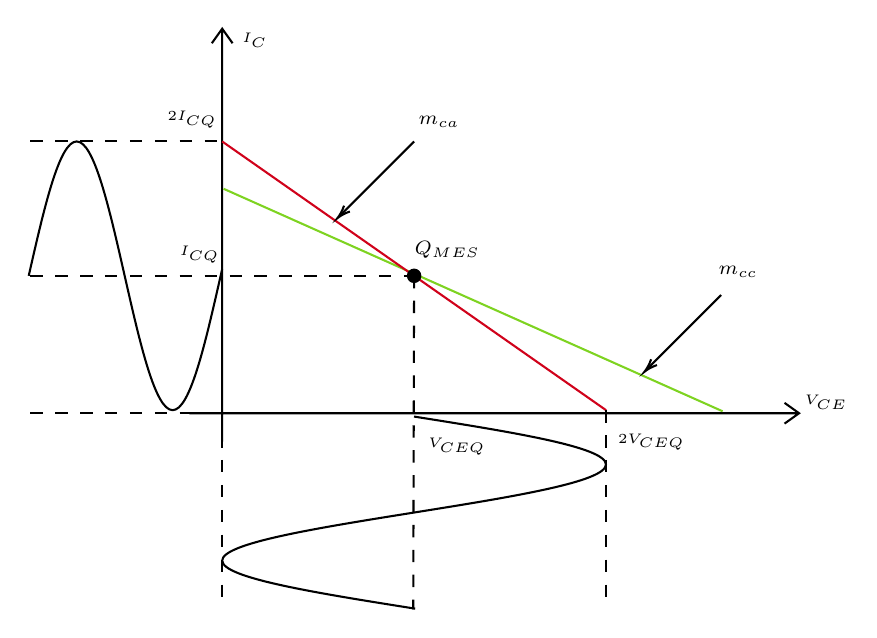
\begin{tikzpicture}[x=0.75pt,y=0.75pt,yscale=-1,xscale=1]
    %uncomment if require: \path (0,538); %set diagram left start at 0, and has height of 538
    
    %Shape: Axis 2D [id:dp5849296416796758] 
    \draw  (178.6,264.42) -- (472.39,264.42)(194.46,79.16) -- (194.46,278.05) (465.39,259.42) -- (472.39,264.42) -- (465.39,269.42) (189.46,86.16) -- (194.46,79.16) -- (199.46,86.16)  ;
    %Straight Lines [id:da0025452687883318337] 
    \draw [color={rgb, 255:red, 126; green, 211; blue, 33 }  ,draw opacity=1 ][fill={rgb, 255:red, 126; green, 211; blue, 33 }  ,fill opacity=1 ]   (195.14,156.28) -- (435.55,263.48) ;
    %Straight Lines [id:da4207709647475807] 
    \draw [color={rgb, 255:red, 208; green, 2; blue, 27 }  ,draw opacity=1 ]   (194.45,133.48) -- (379.39,262.94) ;
    %Shape: Ellipse [id:dp6638447632450213] 
    \draw  [fill={rgb, 255:red, 0; green, 0; blue, 0 }  ,fill opacity=1 ] (283.94,198.21) .. controls (283.94,196.57) and (285.27,195.23) .. (286.92,195.23) .. controls (288.57,195.23) and (289.9,196.57) .. (289.9,198.21) .. controls (289.9,199.86) and (288.57,201.19) .. (286.92,201.19) .. controls (285.27,201.19) and (283.94,199.86) .. (283.94,198.21) -- cycle ;
    %Shape: Wave [id:dp2756289016932214] 
    \draw   (101.24,198.21) .. controls (108.78,165.05) and (115.99,133.48) .. (124.35,133.48) .. controls (132.72,133.48) and (139.93,165.05) .. (147.47,198.21) .. controls (155.01,231.37) and (162.22,262.94) .. (170.59,262.94) .. controls (178.96,262.94) and (186.17,231.37) .. (193.71,198.21) .. controls (193.95,197.13) and (194.2,196.04) .. (194.45,194.96) ;
    %Straight Lines [id:da5275896058426159] 
    \draw [line width=0.75]  [dash pattern={on 4.5pt off 4.5pt}]  (101.98,133.48) -- (194.45,133.48) ;
    %Straight Lines [id:da5594786228796592] 
    \draw [line width=0.75]  [dash pattern={on 4.5pt off 4.5pt}]  (101.99,264.42) -- (194.46,264.42) ;
    %Straight Lines [id:da07986632106139901] 
    \draw [line width=0.75]  [dash pattern={on 4.5pt off 4.5pt}]  (101.98,198.21) -- (286.92,198.21) ;
    %Straight Lines [id:da7967798088876819] 
    \draw [line width=0.75]  [dash pattern={on 4.5pt off 4.5pt}]  (286.92,198.21) -- (286.51,358.87) ;
    %Shape: Wave [id:dp6181760713700251] 
    \draw   (286.88,266.02) .. controls (334.25,273.53) and (379.35,280.72) .. (379.35,289.09) .. controls (379.36,297.46) and (334.27,304.69) .. (286.91,312.26) .. controls (239.54,319.82) and (194.45,327.06) .. (194.46,335.42) .. controls (194.46,343.79) and (239.56,350.98) .. (286.93,358.49) .. controls (287.09,358.52) and (287.25,358.54) .. (287.42,358.57) ;
    %Straight Lines [id:da23476967040469132] 
    \draw  [dash pattern={on 4.5pt off 4.5pt}]  (379.39,262.94) -- (379.39,355.41) ;
    %Straight Lines [id:da643777299413971] 
    \draw  [dash pattern={on 4.5pt off 4.5pt}]  (194.45,262.94) -- (194.45,355.41) ;
    %Straight Lines [id:da5509689272628648] 
    \draw    (286.92,133.48) -- (251.34,169.06) ;
    \draw [shift={(249.93,170.47)}, rotate = 315] [color={rgb, 255:red, 0; green, 0; blue, 0 }  ][line width=0.75]    (6.56,-1.97) .. controls (4.17,-0.84) and (1.99,-0.18) .. (0,0) .. controls (1.99,0.18) and (4.17,0.84) .. (6.56,1.97)   ;
    %Straight Lines [id:da7225229987184748] 
    \draw    (434.87,207.46) -- (399.3,243.03) ;
    \draw [shift={(397.88,244.45)}, rotate = 315] [color={rgb, 255:red, 0; green, 0; blue, 0 }  ][line width=0.75]    (6.56,-1.97) .. controls (4.17,-0.84) and (1.99,-0.18) .. (0,0) .. controls (1.99,0.18) and (4.17,0.84) .. (6.56,1.97)   ;
    
    % Text Node
    \draw (292.24,275.1) node [anchor=north west][inner sep=0.75pt]  [font=\tiny] [align=left] {$\displaystyle V_{CEQ}$};
    % Text Node
    \draw (172.55,182.55) node [anchor=north west][inner sep=0.75pt]  [font=\tiny] [align=left] {$\displaystyle I_{CQ}$};
    % Text Node
    \draw (202.71,79.9) node [anchor=north west][inner sep=0.75pt]  [font=\tiny] [align=left] {$\displaystyle I_{C}$};
    % Text Node
    \draw (473.73,254.25) node [anchor=north west][inner sep=0.75pt]  [font=\tiny] [align=left] {$\displaystyle V_{CE}$};
    % Text Node
    \draw (287.64,119.68) node [anchor=north west][inner sep=0.75pt]  [font=\scriptsize] [align=left] {$\displaystyle m_{ca}$};
    % Text Node
    \draw (432.14,192.26) node [anchor=north west][inner sep=0.75pt]  [font=\scriptsize] [align=left] {$\displaystyle m_{cc}$};
    % Text Node
    \draw (383.71,272.76) node [anchor=north west][inner sep=0.75pt]  [font=\tiny] [align=left] {$\displaystyle 2V_{CEQ}$};
    % Text Node
    \draw (166.67,117.46) node [anchor=north west][inner sep=0.75pt]  [font=\tiny] [align=left] {$\displaystyle 2I_{CQ}$};
    % Text Node
    \draw (285.64,180.08) node [anchor=north west][inner sep=0.75pt]  [font=\scriptsize] [align=left] {$\displaystyle Q_{MES}$};
    \end{tikzpicture}
    \caption{gráfica punto $Q_{MES}$.}
    \label{fig:gráfica-mes}
\end{figure}

\section{Cálculo de R1 y R2}
    % Copiar aquí el planteo y los datos (RE, RC, RL, elección de transistor y VCC)
    Los datos iniciales con los que se cuenta son:
    \begin{itemize}
        \item $R_E = 180\Omega$
        \item $R_C = 1.2K\Omega$
        \item $R_L = 1K\Omega$
        \item $V_{CC} = 12V$
    \end{itemize}
    Adicionalmente, se ha elegido un transistor modelo BC337-40 con un $\beta = 484$, valor que fue medido con un
    multímetro.
    Teniendo esto en cuenta, se puede comenzar aplicando teorema de Thévenin a la red de entrada del circuito
    \ref{fig:amplificador}, obteniendo el circuito de la figura \ref{fig:malla-entrada}.
    
    \begin{figure}[!ht]
        \centering
        \begin{minipage}{0.4\textwidth}
            \centering
            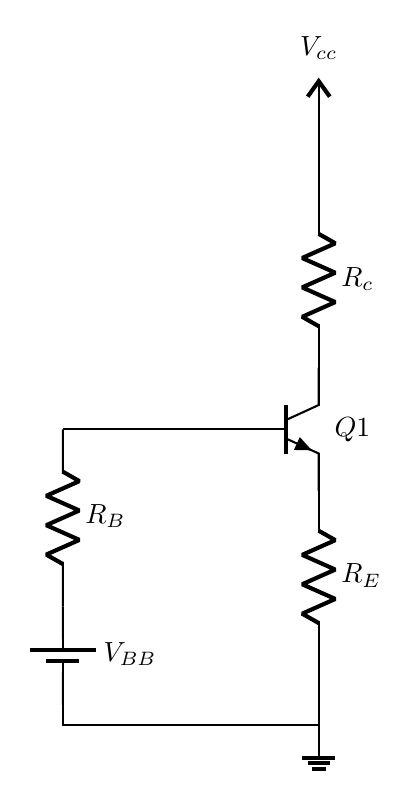
\begin{tikzpicture}
                \node[npn](N1) at (1.59, 2){} node[anchor=west] at (N1.text){$Q1$};
                \draw (1.59, 1.25) to[american resistor, l={$R_E$}] (1.59, -1);
                \draw (1.59, 5.02) to[american resistor, l={$R_c$}] (1.59, 2.77);
                \draw (1.59, -1) -| (1.59, -1.25);
                \node[vcc](N2) at (1.59, 6){} node[anchor=south] at (N2.text){$V_{cc}$};
                \draw (1.59, 5.25) -| (1.59, 6);
                \node[ground] at (1.59, -1.75){};
                \draw (1.59, -1.25) -| (1.59, -1.75);
                \draw (-1.66, 2) to[american resistor, l={$R_B$}] (-1.66, -0.25);
                \draw (-1.66, -0.25) to[battery1, l={$V_{BB}$}] (-1.66, -1.5);
                \draw (-1.66, 2) -| (0.75, 2);
                \draw (-1.66, -1.5) -| (-1.66, -1.75) -- (1.59, -1.75);
                \draw (1.59, 5.02) -| (1.59, 5.25);
            \end{tikzpicture}
            \caption{Malla de entrada simplificada por Thévenin.}
            \label{fig:malla-entrada}
        \end{minipage}%
        \begin{minipage}{0.4\textwidth}
            \centering
            Donde $R_{B}$ la resistencia equivalente y $V_{BB}$ es la tensión de Thévenin:
            \begin{align*}
                R_{B} &= R_1||R_2=\frac{R_1 R_2}{R_1 + R_2} \\
                V_{BB} &= V_{CC} \cdot \frac{R_1}{R_1 + R_2} \\
            \end{align*}
        \end{minipage}
    \end{figure}

    Aplicando LKV a la malla de entrada:

    \begin{align*}
        V_{BB} - I_{BQ} R_B - V_{BEQ} - I_{CQ} R_E &= 0 \\
        V_{BB} - \frac{I_{CQ}}{\beta} R_B - V_{BEQ} - I_{CQ} R_E &= 0 \\
        I_{CQ} &= \frac{V_{BB} - V_{BEQ}}{R_E + \frac{R_B}{\beta}} 
    \end{align*}

Considerando el siguiente criterio de diseño: 

\begin{equation*}
    R_E  \gg \frac{R_b}{\beta} \therefore R_E = 10\frac{R_B}{\beta} \therefore \frac{R_B}{\beta} = \frac{R_E}{10}
\end{equation*}

Se tiene:

\begin{equation*}
    I_{CQ} = \frac{V_{BB} - V_{BEQ}} {R_E + \frac{R_E}{10}}
\end{equation*}


    

\subsection{Teorema de Thévenin en red de entrada}
    \subsection{Análisis de malla de entrada}
    \subsection{Criterios de diseño y fórmulas generales}
    \subsection{Cálculo final de R1 y R2} \label{section:calc_r1_r2}
  \section{Simulación}
    \subsection{Simulación con valores de diseño}
    \subsection{Simulación con valores normalizados}
    \subsection{Comparación con cálculos analíticos}
  \section{Implementación y mediciones}
    \subsection{Mediciones en circuito implementado}
    \subsection{Consideraciones de medición}
    \subsection{Cálculo de parámetros a partir de mediciones}

\chapter{Análisis y trazado de rectas de carga}
  Partiendo de los valores de R1 y R2 obtenidos en la seccion \ref{section:calc_r1_r2}, se busco encontrar los valores
  comerciales mas proximos a los obtenidos analiticamente, y que no afecten significativamente el punto Q. La variacion
  maxima permitida es del 10\%.
  \begin{figure}[!ht]
    \centering
    \begin{minipage}{0.7\textwidth}
      \resizebox{\textwidth}{!}{
      \begin{tikzpicture}
        \node[npn](N1) at (9.25, 5.75){} node[anchor=west] at (N1.text){$Q1$};
        \draw (7, 5) to[american resistor, l={$R_1$}] (7, 2.75);
        \draw (7, 5.75) to[capacitor, l={$C_1$}] (3, 5.75);
        \draw (7, 5.75) -- (8.41, 5.75);
        \draw (9.25, 5) to[american resistor, l={$R_E$}] (9.25, 2.75);
        \draw (3, 5.75) to[sinusoidal voltage source, l={$v_i$}] (3, 2.5);
        \draw (7, 8.75) to[american resistor, l={$R_2$}, name=R1] (7, 6.5);
        \draw (9.25, 8.77) to[american resistor, l={$R_C$}] (9.25, 6.52);
        \draw (7, 5) -| (7, 6.5);
        \draw (11, 5) to[capacitor, l={$C_E$}] (11, 2.75);
        \draw (9.25, 5) -- (11, 5);
        \draw (7, 8.75) -| (7, 9) -| (9.25, 8.77);
        \draw (11, 2.75) |- (7, 2.5) -| (7, 2.75);
        \draw (9.25, 2.75) -| (9.25, 2.5);
        \draw (3, 2.5) -- (7, 2.5);
        \draw (10.25, 6.5) to[capacitor, l={$C_2$}] (13, 6.5);
        \draw (13.75, 5.5) to[american resistor, l={$R_L$}] (13.75, 3.25);
        \draw (13.75, 6.5) -| (13.75, 5.5);
        \draw (11, 2.5) -| (13.75, 3.25);
        \node[vcc](N2) at (9.25, 9.75){} node[anchor=south] at (N2.text){$V_{cc}$};
        \draw (9.25, 9) -| (9.25, 9.75);
        \node[ground] at (9.25, 2){};
        \draw (9.25, 2.5) -| (9.25, 2);
        \draw (10.25, 6.5) -- (9.25, 6.5);
        \draw (13, 6.5) -- (13.75, 6.5);
      \end{tikzpicture}
      }
    \end{minipage}
    \begin{minipage}{0.2\textwidth}
      \centering
      \begin{align*}
        R_1 &= 10K \Omega\\
        R_2 &= 54K4 \Omega\\
        R_C &= 1K2 \Omega\\
        R_E &= 180 \Omega\\
        R_L &= 1K \Omega\\
        V_{CC} &= 12V\\
        \beta &= 484
      \end{align*}
    \end{minipage}
    \caption{Amplificador emisor común con resistencias normalizadas.}
  \end{figure}

  No logramos encontrar un conjunto de resistencias normalizadas que nos permitiesen estar dentro del margen de
  tolerancia del punto Q, asi que fijamos la $R_1$ al valor normalizado mas cercano, y jugamos con la $R_2$ para
  encontrar un serie de resistencias normalizadas. Al final, quedamos con un serie de 3K3 y 51K1. Se procede a corroborar
  si el punto Q esta dentro del 10\% del calculado con los valores analiticos de las resistencias, reemplazando su
  valor en las ecuaciones \warn ICQ REF y VCEQ REF.

  \begin{figure}[!ht]
    \centering
    \begin{minipage}{0.49\textwidth}
      \begin{align*}
        I_{CQ} &= \frac{V_{BB} - V_{BE}}{\frac{R_B}{\beta} + R_E}\\[6pt]
        I_{CQ} &= \frac{\frac{R_1}{R_1 + R_2} V_{CC} - V_{BE}}{\frac{R_1//R_2}{\beta} + R_E}\\[6pt]
        I_{CQ} &= \frac{1.86V - 1.7V}{\frac{8444.79 \Omega}{484} + 180 \Omega}\\[6pt]
        I_{CQ} &= 5.9 mA
      \end{align*}
    \end{minipage}
    \begin{minipage}{0.49\textwidth}
      \begin{align*}
        V_{CEQ} &= V_{CC} - I_{CQ} \left(R_C + R_E \right)\\[6pt]
        V_{CEQ} &= 12V - 5.9mA \left(1K2 \Omega + 180 \Omega \right)\\[6pt]
        V_{CEQ} &= 3.84V
      \end{align*}
    \end{minipage}
  \end{figure}

  Como se puede ver, el $I_{CQ}$ esta dentro del 10\% del $I_{CQ mes}$ calculado analiticamente, pero no para el
  $V_{CEQ}$. Corroborando con la simulacion en LTSpice, los valores obtenidos son parecidos, pero estos si caen dentro
  del 10\% del $I_{CQ mes}$ y $V_{CEQ mes}$ como se puede ver en la figura \ref{fig:pto_q_normalizado}. Esta diferencia
  puede ser provocada por asumir que $I_E \approx I_C$ y/o la omision de las corrientes de fuga.

  \begin{figure}[!ht]
    \centering
    \includegraphics[width=.9\textwidth]{images/pto_q_normalizado.png}
    \caption{simulacion del punto Q con resistencias normalizadas.}
    \label{fig:pto_q_normalizado}
  \end{figure}

  \section{Rectas de Carga}
    Para el trazado de las rectas de carga, se parte del analisis de la malla de salida con LKV. Para el analisis en CC,
    los capacitores pueden ser considerados como circuitos abiertos debido a que su impedancia en CC es demasiado alta.
    En la figura \ref{fig:recta_cc} puede ver el circuito resultante y el analisis con LKV.
    \begin{figure}[!ht]
      \centering
      \begin{minipage}{0.49\textwidth}
        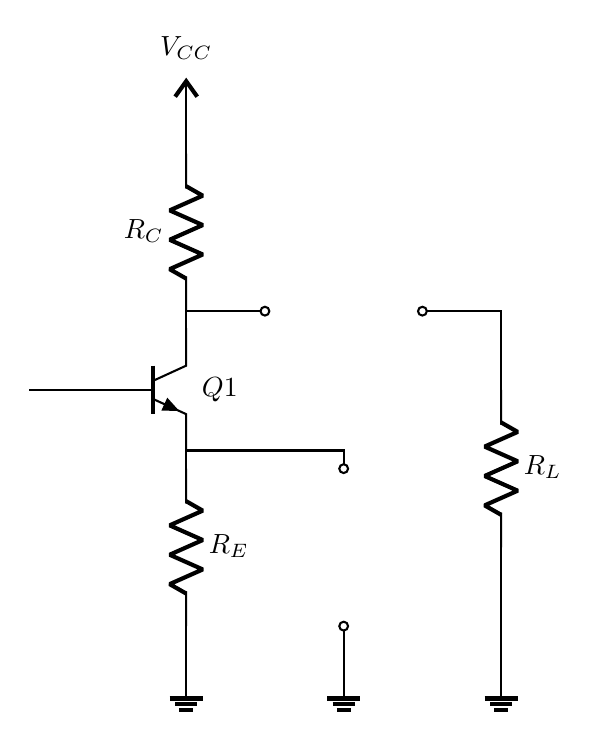
\begin{tikzpicture}
          % Paths, nodes and wires:
          \node[npn](N1) at (1, 0){} node[anchor=west] at (N1.text){$Q1$};
          \draw (1, 1) to[american resistor, l={$R_C$}] (1, 3);
          \draw (1, -1) to[american resistor, l={$R_E$}] (1, -3);
          \node[ground] at (1, -3.5){};
          \node[vcc](N2) at (1, 3.5){} node[anchor=south] at (N2.text){$V_{CC}$};
          \draw (1, 3.5) -| (1, 3);
          \draw (1, 1) -| (1, 0.77);
          \draw (1, -0.77) -| (1, -1);
          \draw (1, -3) -| (1, -3.5);
          \draw (0.16, 0) -- (-1, -0);
          \draw (5, -0) to[american resistor, l={$R_L$}] (5, -2);
          \node[ground] at (5, -3.5){};
          \draw (5, -3.5) -- (5, -2);
          \draw (5, -0) -| (5, 1) -- (4, 1);
          \draw (2, 1) -- (1, 1);
          \draw (3, -1) |- (1, -0.77);
          \draw (3, -3) -| (3, -3.5);
          \node[ground] at (3, -3.5){};
          \node[ocirc] at (2, 1){};
          \node[ocirc] at (4, 1){};
          \node[ocirc] at (3, -1){};
          \node[ocirc] at (3, -3){};
        \end{tikzpicture}
      \end{minipage}
      \begin{minipage}{0.49\textwidth}
        \begin{align*}
          0 &= V_{CC} - V_{R_C} - v_{CE} - V_{R_E}\\[6pt]
          v_{CE} &= V_{CC} - R_C i_C - R_E i_E \qquad\to i_E \approx i_C\\[6pt]
          v_{CE} &= V_{CC} - i_C (R_C + R_E)
        \end{align*}
      \end{minipage}
      \caption{analisis para la recta de carga en CC.}
      \label{fig:recta_cc}
    \end{figure}

    Queda asi determinada la ecuacion de la recta de carga en CC para el BJT en configuracion emisor comun.

    Para el analisis de la recta de carga en CA, se procede de la misma manera. En este caso, los capacitores actuan
    como cables debido a la baja impedancia en CA. Tambien, las fuentes de alimentacion de CC actuan como
    "cortoricuitos" a masa, por lo que son reemplazadas correspondientemente. Puede revisar la figura \ref{fig:recta_ca}
    con el circuito resultante y el analisis con LKV.
    \begin{figure}[H]
      \centering
      \begin{minipage}{0.49\textwidth}
        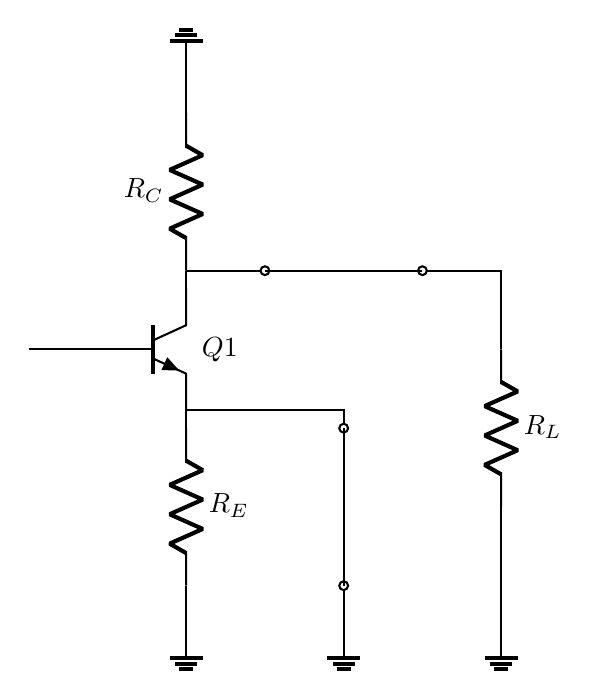
\begin{tikzpicture}
          % Paths, nodes and wires:
          \node[npn](N1) at (1, 0){} node[anchor=west] at (N1.text){$Q1$};
          \draw (1, 1) to[american resistor, l={$R_C$}] (1, 3);
          \draw (1, -1) to[american resistor, l={$R_E$}] (1, -3);
          \node[ground] at (1, -3.5){};
          \draw (1, 3.5) -| (1, 3);
          \draw (1, 1) -| (1, 0.77);
          \draw (1, -0.77) -| (1, -1);
          \draw (1, -3) -| (1, -3.5);
          \draw (0.16, 0) -- (-1, -0);
          \draw (5, -0) to[american resistor, l={$R_L$}] (5, -2);
          \node[ground] at (5, -3.5){};
          \draw (5, -3.5) -- (5, -2);
          \draw (5, -0) -| (5, 1) -- (4, 1);
          \draw (2, 1) -- (1, 1);
          \draw (3, -1) |- (1, -0.77);
          \draw (3, -3) -| (3, -3.5);
          \node[ground] at (3, -3.5){};
          \node[ocirc] at (2, 1){};
          \node[ocirc] at (4, 1){};
          \node[ocirc] at (3, -1){};
          \node[ocirc] at (3, -3){};
          \node[ground, xscale=-1, yscale=-1] at (1, 3.5){};
          \draw (2, 1) -- (4, 1);
          \draw (3, -1) -- (3, -3);
        \end{tikzpicture}
      \end{minipage}
      \begin{minipage}{0.49\textwidth}
        \begin{align*}
          v_{CE} &= V_{CC}' - i_C (R_C//R_L),\\[6pt]
          V_{CC}' &= V_{CEQ mes} + I_{CQ mes} (R_C//R_L)
        \end{align*}
      \end{minipage}
      \caption{analisis para la recta de carga en CA.}
      \label{fig:recta_ca}
    \end{figure}

    Para trazar las rectas, podemos proceder sacando sus intersecciones en los ejes. Para CC:
    \begin{figure}[H]
      \centering
      \begin{minipage}[t]{0.49\textwidth}
        Para $V_{CE} = 0$:
        \begin{align*}
          0 =& V_{CC} - i_C(R_C + R_E)\\[6pt]
          i_C =& \frac{V_{CC}}{R_C + R_E}\\[6pt]
          i_C =& 8.695mA
        \end{align*}
      \end{minipage}
      \begin{minipage}[t]{0.49\textwidth}
        Para $i_C = 0$:
        \begin{align*}
          V_{CE} = V_{CC}\\[6pt]
          V_{CE} = 12V
        \end{align*}
      \end{minipage}
    \end{figure}

    Para CA:
    \begin{figure}[H]
      \centering
      \begin{minipage}[t]{0.49\textwidth}
        Para $V_{CE} = 0$:
        \begin{align*}
          0 =& V_{CC}' - i_C(R_C//R_L)\\[6pt]
          i_C =& \frac{V_{CEQ mes} + I_{CQ mes} (R_C//R_L)}{R_C//R_L}\\[6pt]
          i_C =& 12.94mA
        \end{align*}
      \end{minipage}
      \begin{minipage}[t]{0.49\textwidth}
        Para $i_C = 0$:
        \begin{align*}
          V_{CE} &= V_{CC}'\\[6pt]
          V_{CE} &= V_{CEQ mes} + I_{CQ mes} (R_C//R_L)\\[6pt]
          V_{CE} &= 7.05V
        \end{align*}
      \end{minipage}
    \end{figure}

    Por lo que la recta de carga nos quedaria como la de la figura \ref{fig:recta_carga}.
    \begin{figure}[!ht]
      \centering
      \begin{minipage}{0.45\textwidth}
        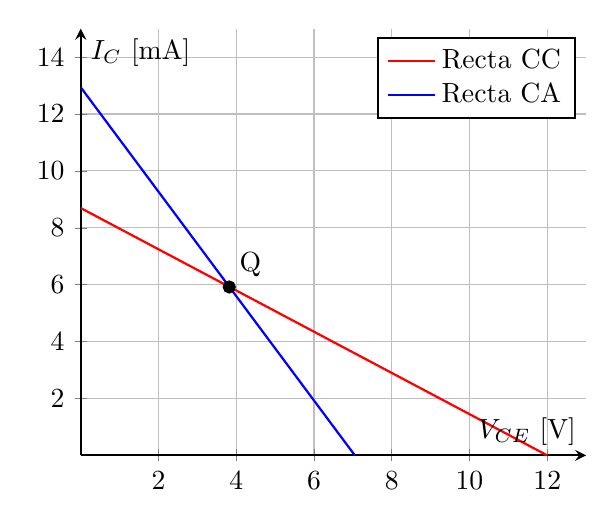
\begin{tikzpicture}
          \begin{axis}[
              axis lines=middle,
              xlabel={$V_{CE}$ [V]},
              ylabel={$I_C$ [mA]},
              xmin=0, xmax=13,
              ymin=0, ymax=15,
              grid=both,
              width=8cm,
              height=7cm,
              xtick={0,2,...,12},
              ytick={0,2,...,14},
          ]
            % Recta de CC: pasa por (0,8.695) y (12,0)
            \addplot[red, thick] coordinates {(0,8.695) (12,0)};
            \addlegendentry{Recta CC}
            % Recta de CA: pasa por (0,12.94) y (7.05,0)
            \addplot[blue, thick] coordinates {(0,12.94) (7.05,0)};
            \addlegendentry{Recta CA}
            % Punto Q
            \addplot[only marks, mark=*] coordinates {(3.82,5.92)};
            \node[above right] at (axis cs:3.82,5.92) {Q};
          \end{axis}
        \end{tikzpicture}
      \end{minipage}
      \begin{minipage}{0.54\textwidth}
        \begin{gather*}
          v_{CE_{CC}} = v_{CE_{CA}}\\[6pt]
          V_{CC} - i_C (R_C + R_E) = V_{CC}' - i_C (R_C//R_L)\\[6pt]
          i_C = \frac{V_{CC} - V_{CEQ mes} - I_{CQ mes} (R_C//R_L)}{R_C + R_E - R_C//R_L}\\[6pt]
          i_{CQ} = 5.92mA \qquad \to v_{CEQ} = 3.82V
        \end{gather*}
      \end{minipage}
      \caption{recta de carga con punto Q en interseccion.}
      \label{fig:recta_carga}
    \end{figure}

    De esta forma, corroboramos que el punto Q esta donde intersecan ambas rectas de carga. Cabe destacar que para todos
    los calculos, se utilizadon los valores calculados del punto Q con las resistencias normalizadas.
  \section{Obtención experimental de parámetros}
    \subsection{Corrientes en el divisor resistivo}
    \subsection{Verificación de resultados}

\chapter{Mediciones de pequeña señal}
  \section{Análisis teórico (método analítico)}
    \subsection{Circuito híbrido equivalente}
    \subsection{Cálculo de $Z_i$, $Z_o$, $A_i$ y $A_v$}
  \section{Análisis experimental}
    \subsection{Impedancia de entrada}
    \subsection{Ganancia de tensión}
    \subsection{Ganancia de corriente}
    \subsection{Impedancia de salida}


\end{document}
